
\subsubsection{Demonstrator: Thermo-Electric Coupling}
\label{sec:app:specs:thermoelectric:hl-31}

%Thermo Electric coupling in a complex geometry.

\paragraph{Description}

This benchmark models the temperature field and electric current distribution in an high field resistive magnet of the Laboratoire National des Champs Magnétiques Intenses. The magnet consist in a set of 14 copper alloys cylindrical tubes connected 2 by 2 into series by rings. In each tube, the current path is defined by 2 helical cuts of 0.2 mm width. The rings are machined to let water flow in between each tube
in a channel of 0.8 mm. The magnet is operated at 12 MW with an imosed total current of 31 kA. The water flow in the magnet is about 140 l/s. The water cooling of the magnet is modelling by using Robin boundary conditions with parameters derived from classical correlation in thermo-hydraulics.
A more detailled version of the full model is available in \cite{daver2016,Hild2020}. The
model is run with \texttt{thermoelectric} \Feelpp toolbox.

The geometry used in this benchmark performance is illustrated in
\Cref{fig:spec:app-feelpp:hl-31:visualization-geometry}. This is a complex domain
composed of a large number of components, with some very thin parts.

\paragraph{Benchmarking Tools Used}
The benchmark was performed on \textbf{Gaya} supercomputer (see \Cref{sec:arch:gaya}) and \textbf{Discoverer} supercomputer (see
\Cref{sec:arch:eurohpc-ju}).
The performance tools integrated into the \Feelpp-toolboxes framework were used to measure
the execution time.
Moreover, we need to say that we have used several \Feelpp installations
\begin{itemize}
\item \textbf{Gaya} : native application from Ubuntu packages of Jammy OS.
\item \textbf{Discoverer} : Apptainer with \Feelpp SIF image based on Ubuntu
  Noble OS.
\end{itemize}
Note: the \Feelpp version is identical but the dependencies (like Petsc)
which are of course more recent with Noble.

The metrics measured are the execution time of the main components of the simulation. We enumerate these parts in the following:
\begin{itemize}
\item \textbf{Init}: load mesh from filesystem and initialize solid toolbox (finite element context and algebraic data structure)
\item \textbf{Assembly}: calculate and assemble the matrix and rhs values obtained using the finite element method
\item \textbf{Solve}: the linear system by using a preconditioned GMRES.
\item \textbf{PostProcess}: Export on the filesystem a visualization format (EnsighGold) of the
  solution and other fields of interest such as current density and electric field.
\end{itemize}

\begin{figure}[!ht]
  \centering
  \begin{subfigure}[c]{0.49\textwidth}
    \centering
    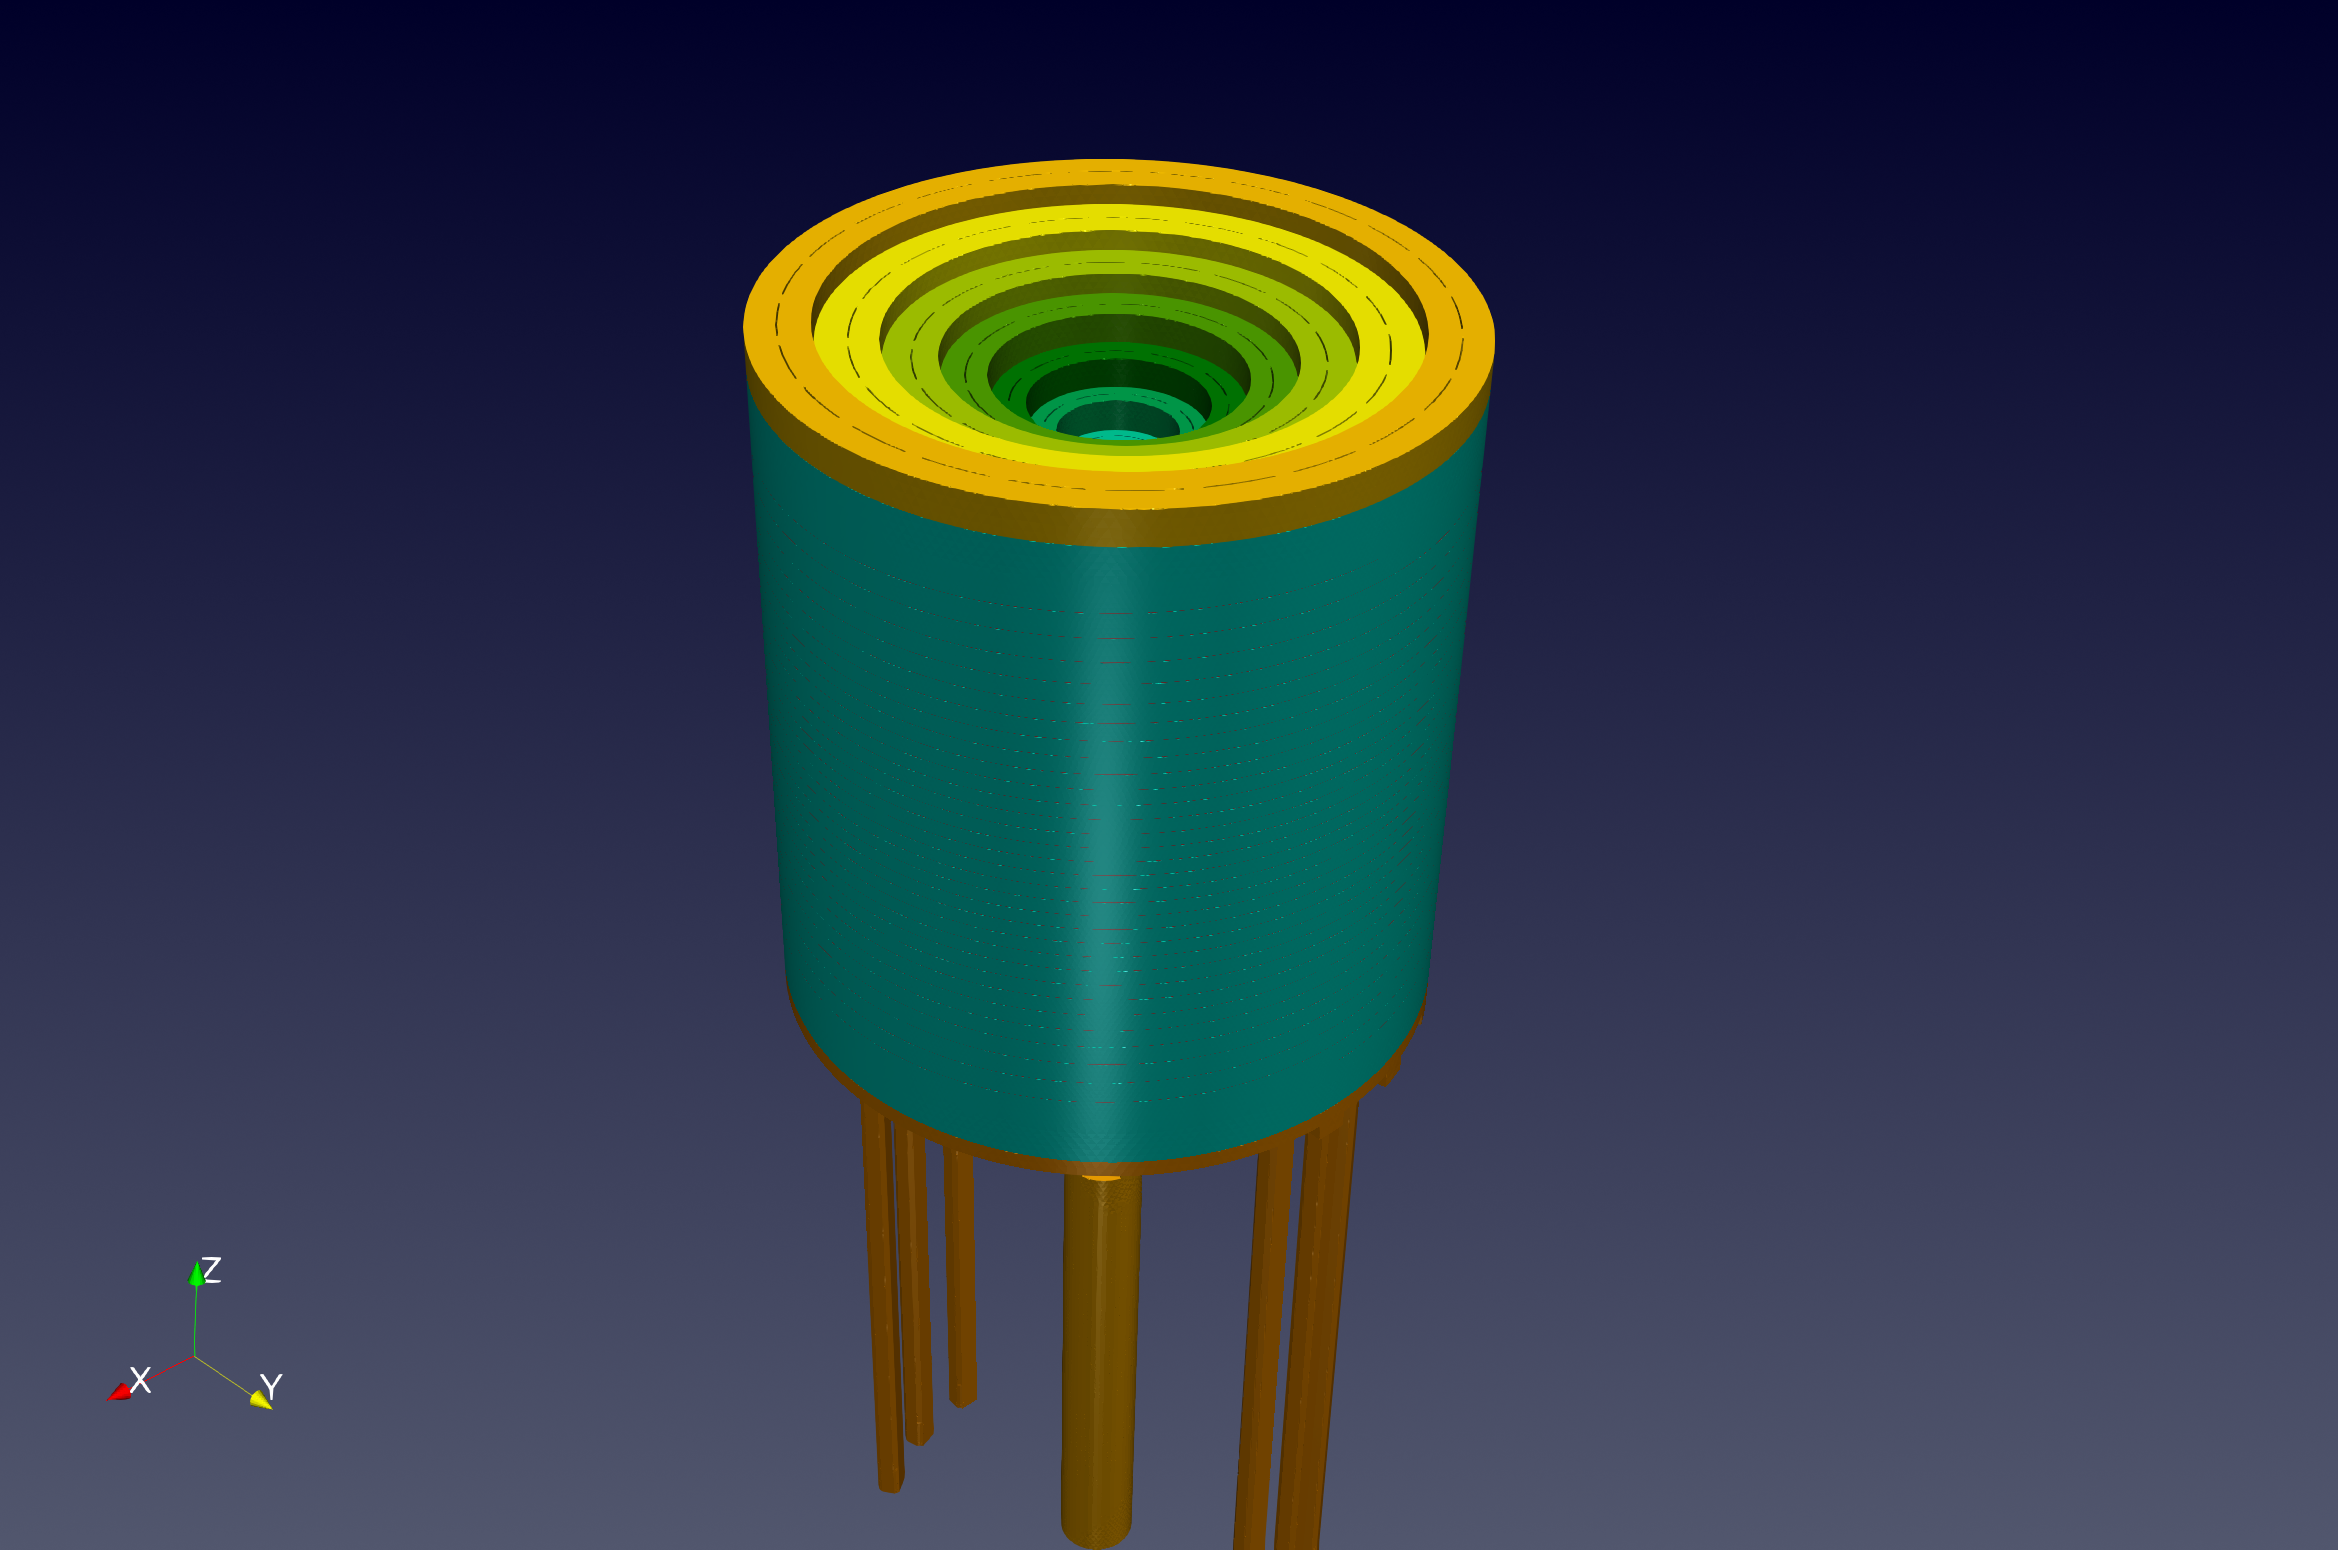
\includegraphics[width=\textwidth]{graphics/feelpp/feelpp-benchmark-HL-31-geo.png}
  \end{subfigure}
  \hfill
  \begin{subfigure}[c]{0.49\textwidth}
    \centering
    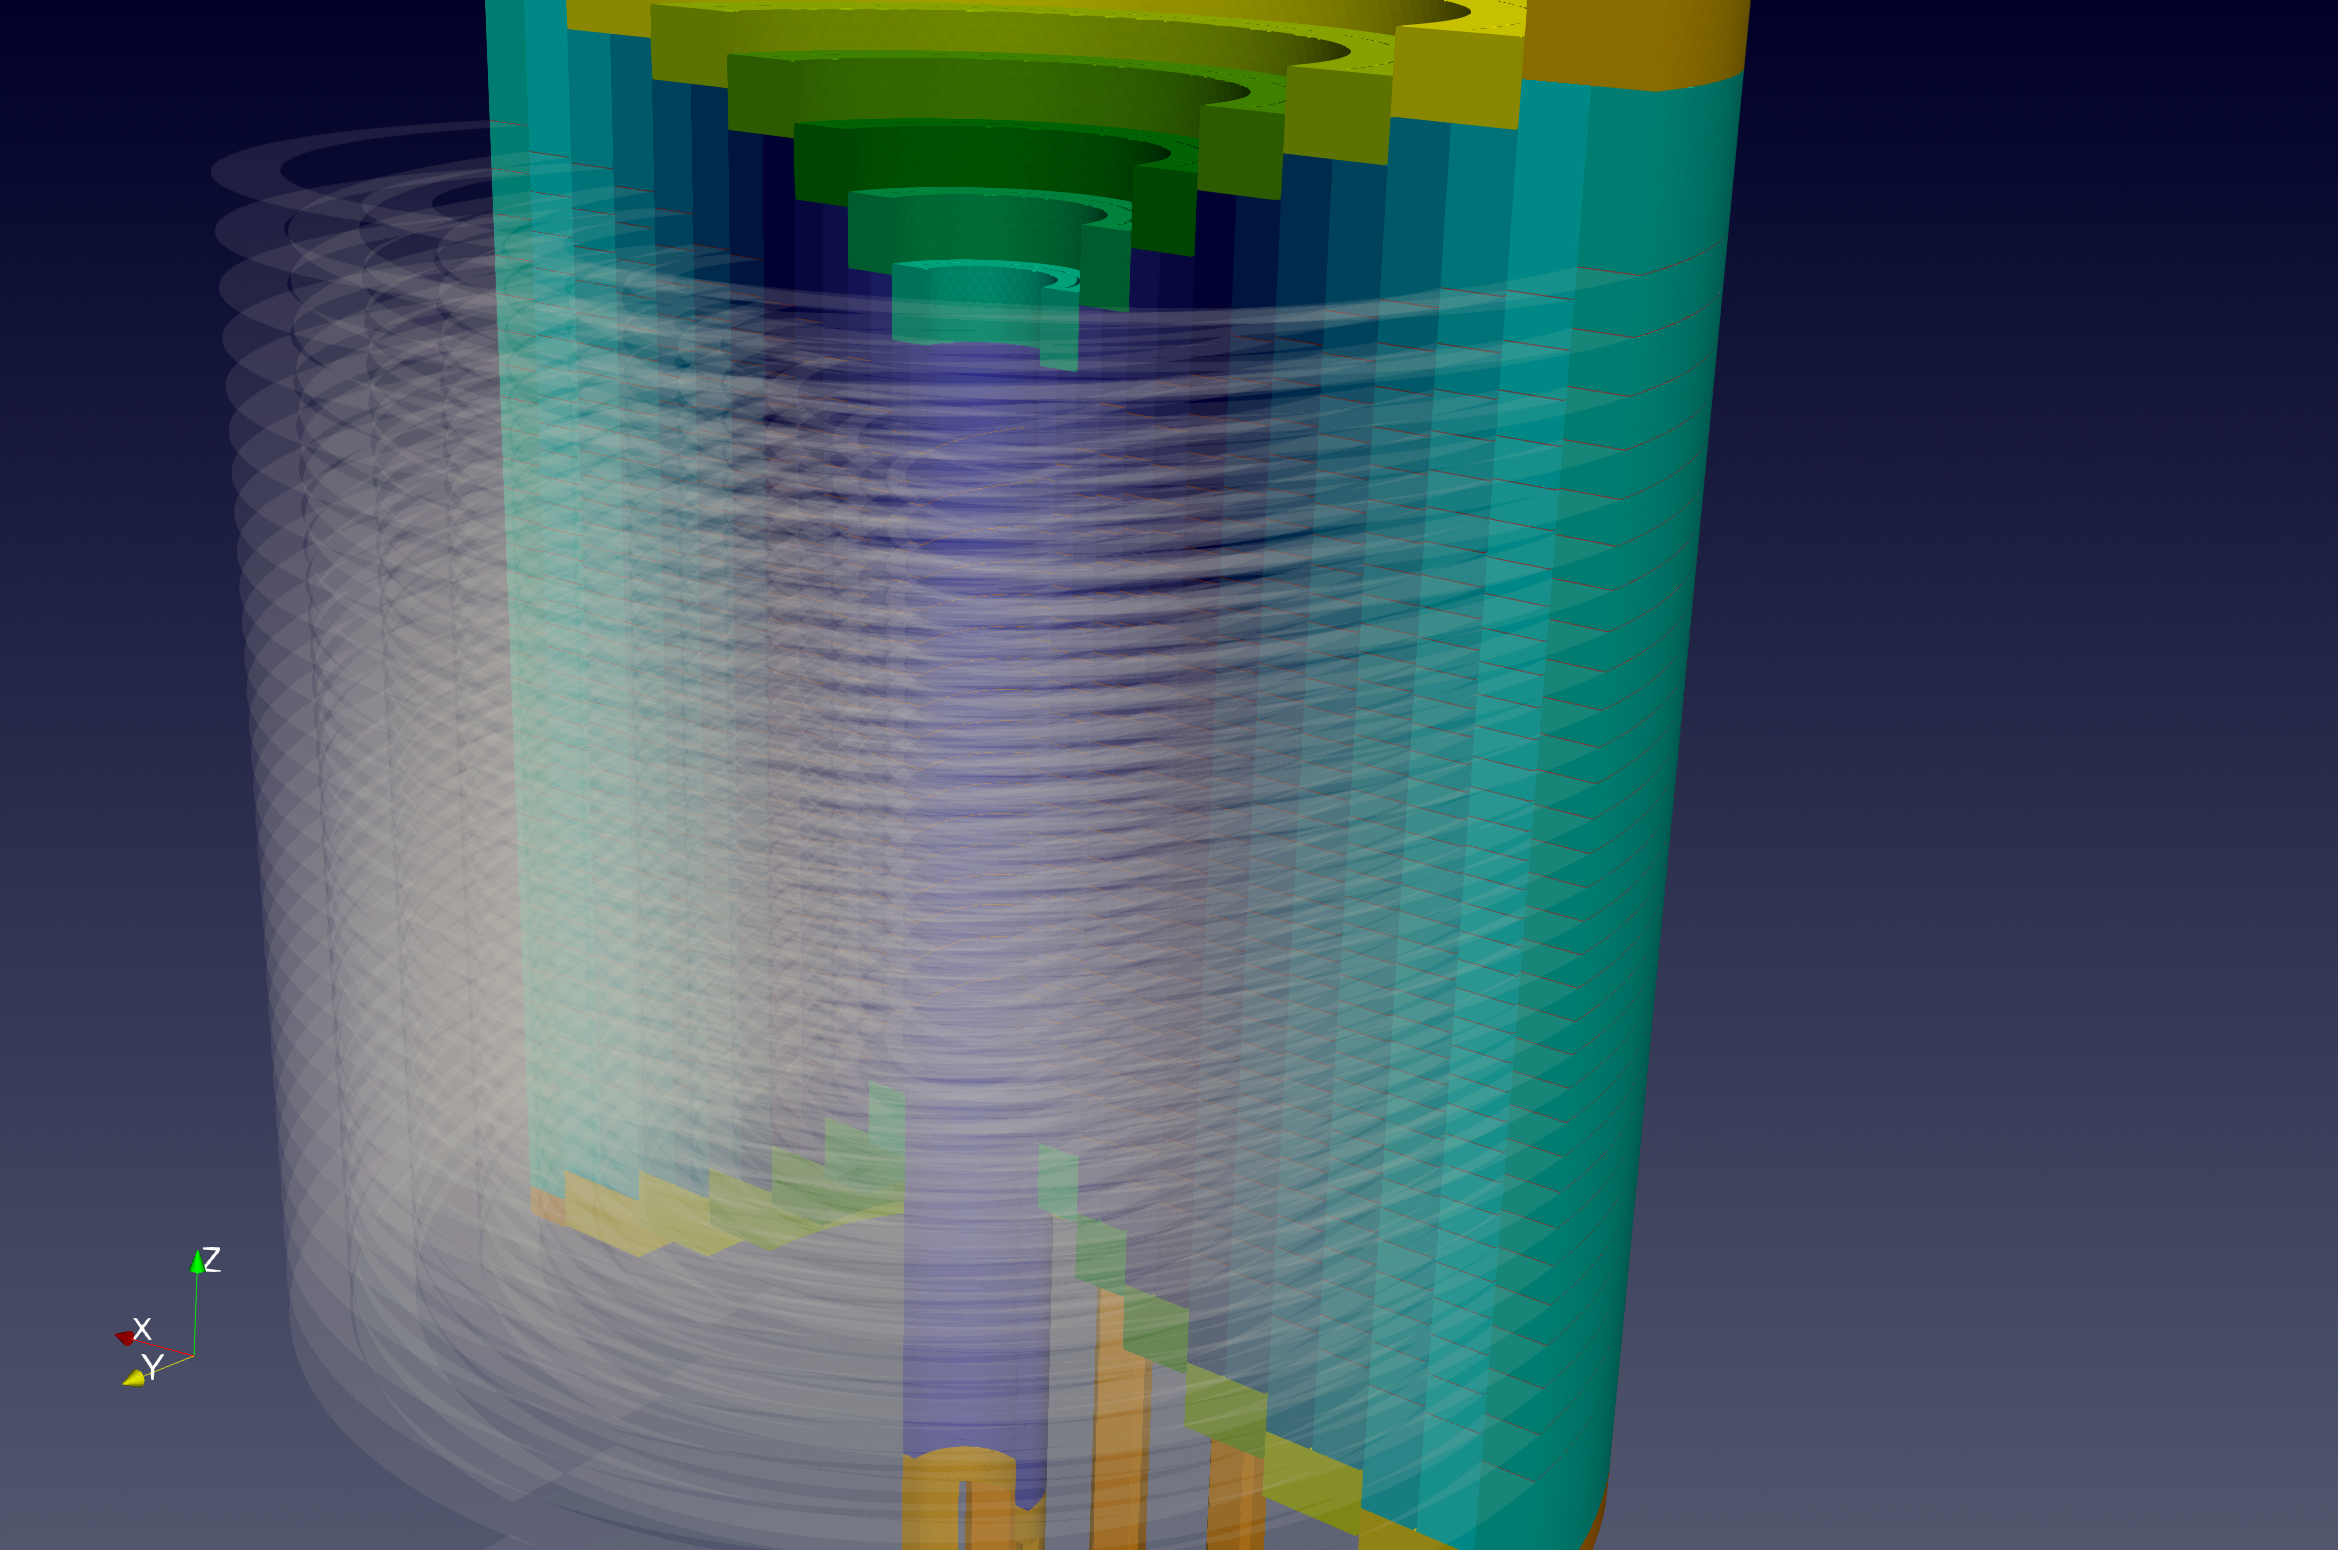
\includegraphics[width=\textwidth]{graphics/feelpp/feelpp-benchmark-HL-31-geo-zoom.png}
  \end{subfigure}
  \caption{HL-31 benchmarks - geometry}
  \label{fig:spec:app-feelpp:hl-31:visualization-geometry}
\end{figure}



\paragraph{Input/Output Dataset Description}

\begin{itemize}
\item \textbf{Input Data:}
  \begin{itemize}
  \item Meshes: We have generated three levels of mesh called M1, M2
    and M3. These meshes are stored in GMSH format. The statistics can be found in
    \Cref{tab:spec:app-feelpp:hl-31:discr_stat}. We have also prepared for
    each mesh level a collection of partitioned mesh.
    The format used is an in-house mesh format of \Feelpp based on
    JSON+HDF5 file type.
    The Gmsh meshes and the partitioned meshes can be found on our Girder
    database management, in the \Feelpp collections.
  \item Setup: Use standard setup of \Feelpp toolboxes. It corresponds to a cfg
    file and JSON file. These config files are present in the Github of feelpp.
  \item[]{\Feelpp distributions}
    \begin{itemize}
    \item SIF image (Apptainer): feelpp:v0.111.0-preview.10-noble-sif  (stored in the Github registry of \Feelpp)
    \item Ubuntu package Jammy (Native) feelpp:v0.111.0-preview.10
    \end{itemize}
  \end{itemize}
\item \textbf{Output Data:} The output includes export visualization files (mesh,
  partitioning, temperature,  elecric potential, current density, electric
  field, ...), the time taken to perform each simulation step and
  some integral quantities such a the total power dissipated by the magnet.
\item \textbf{Data Repository:} All inputdatasets are available in a unistra girder repository (collection HiFiMagnet, HL-31).
\end{itemize}



\begin{table}[h!]
  \centering
  { \setlength{\parindent}{0pt}
    \def\arraystretch{1.25}
    \arrayrulecolor{numpexgray}
    {\fontsize{9}{11}\selectfont
      \begin{tabular}{!{\color{numpexgray}\vrule}c!{\color{numpexgray}\vrule}c!{\color{numpexgray}\vrule}c!{\color{numpexgray}\vrule}c!{\color{numpexgray}\vrule}c!{\color{numpexgray}\vrule}c!{\color{numpexgray}\vrule}c!{\color{numpexgray}\vrule}c!{\color{numpexgray}\vrule}c!{\color{numpexgray}\vrule}}
        \rowcolor{numpexgray}\multicolumn{5}{c!{\color{numpexgray}\vrule}}{\color{white}\bf Mesh properties}
        & \multicolumn{2}{c!{\color{numpexgray}\vrule}}{\color{white}\bf Number of dof (heat)}
        & \multicolumn{2}{c!{\color{numpexgray}\vrule}}{\color{white}\bf Number of dof (electric)} \\
        \rowcolor{numpexgray} {\color{white}\bf Tag} & {\color{white}\bf \# points} & {\color{white}\bf \# edges} & {\color{white}\bf \# faces} & {\color{white}\bf \# elements} & {\color{white}\bf $P_1$} & {\color{white}\bf $P_2$} & {\color{white}\bf $P_1$} & {\color{white}\bf $P_2$} \\
        \texttt{M1} & \pgfmathprintnumber{4306880} & \pgfmathprintnumber{27913534} & \pgfmathprintnumber{46008143} & \pgfmathprintnumber{22401676} & \pgfmathprintnumber{4306880} & \pgfmathprintnumber{32220414} & \pgfmathprintnumber{4302090} & \pgfmathprintnumber{29456526}  \\
        \hline
      \end{tabular}
    }}
  \caption{HL-31 benchmark - Statistics on meshes and number of degrees of freedom with respect
    to finite element approximation}
  \label{tab:spec:app-feelpp:hl-31:discr_stat}
\end{table}

\paragraph{Results Summary}

We can find in \cref{fig:spec:app-feelpp:hl-31:results:visualization-solution} some
examples of 3D visualization that represent fields obtained by solving the
thermoelectric problem. We have the temperature solution and other quantities
evaluated at \textbf{PostProcess} phase such as current density, electric
potential, and electric fields.

The performance analysis has been done in two supercomputers, Gaya and
Discoverer. For each of them, we have run the benchmark with discretizations P1
and P2. About the \Feelpp distribution, we use native Ubuntu Jammy packages for
Gaya, and Apptainer (with Ubuntu) for Discoverer. The results on these machines
are illustrated in
\cref{fig:spec:app-feelpp:hl-31:results:performance_times_M1_gaya} %,fig:feelpp:spec:hl-31:results:performance_times_M1_discoverer
respectively. The measures presented are the time-consuming of simulation
components related to WP1, namely \textbf{Init}, \textbf{Assembly}, and
\textbf{PostProcess}.

In each case analyzed, we have very good scalability, in the sense that we
reduced significantly the execution time by increasing the number of tasks. The
\textbf{Init} phase is the most time-consuming, with a limit quite high compared
to others. This part contains the mesh reading from the disk, which can explain
some bumps sometimes when require many HPC resources.

To conclude, we can say that we successfully ran this benchmark case, and we are
ready to go up to larger problems and more complex modeling.



\begin{figure}[!ht]
  \centering
  \begin{subfigure}[c]{0.49\textwidth}
    \centering
    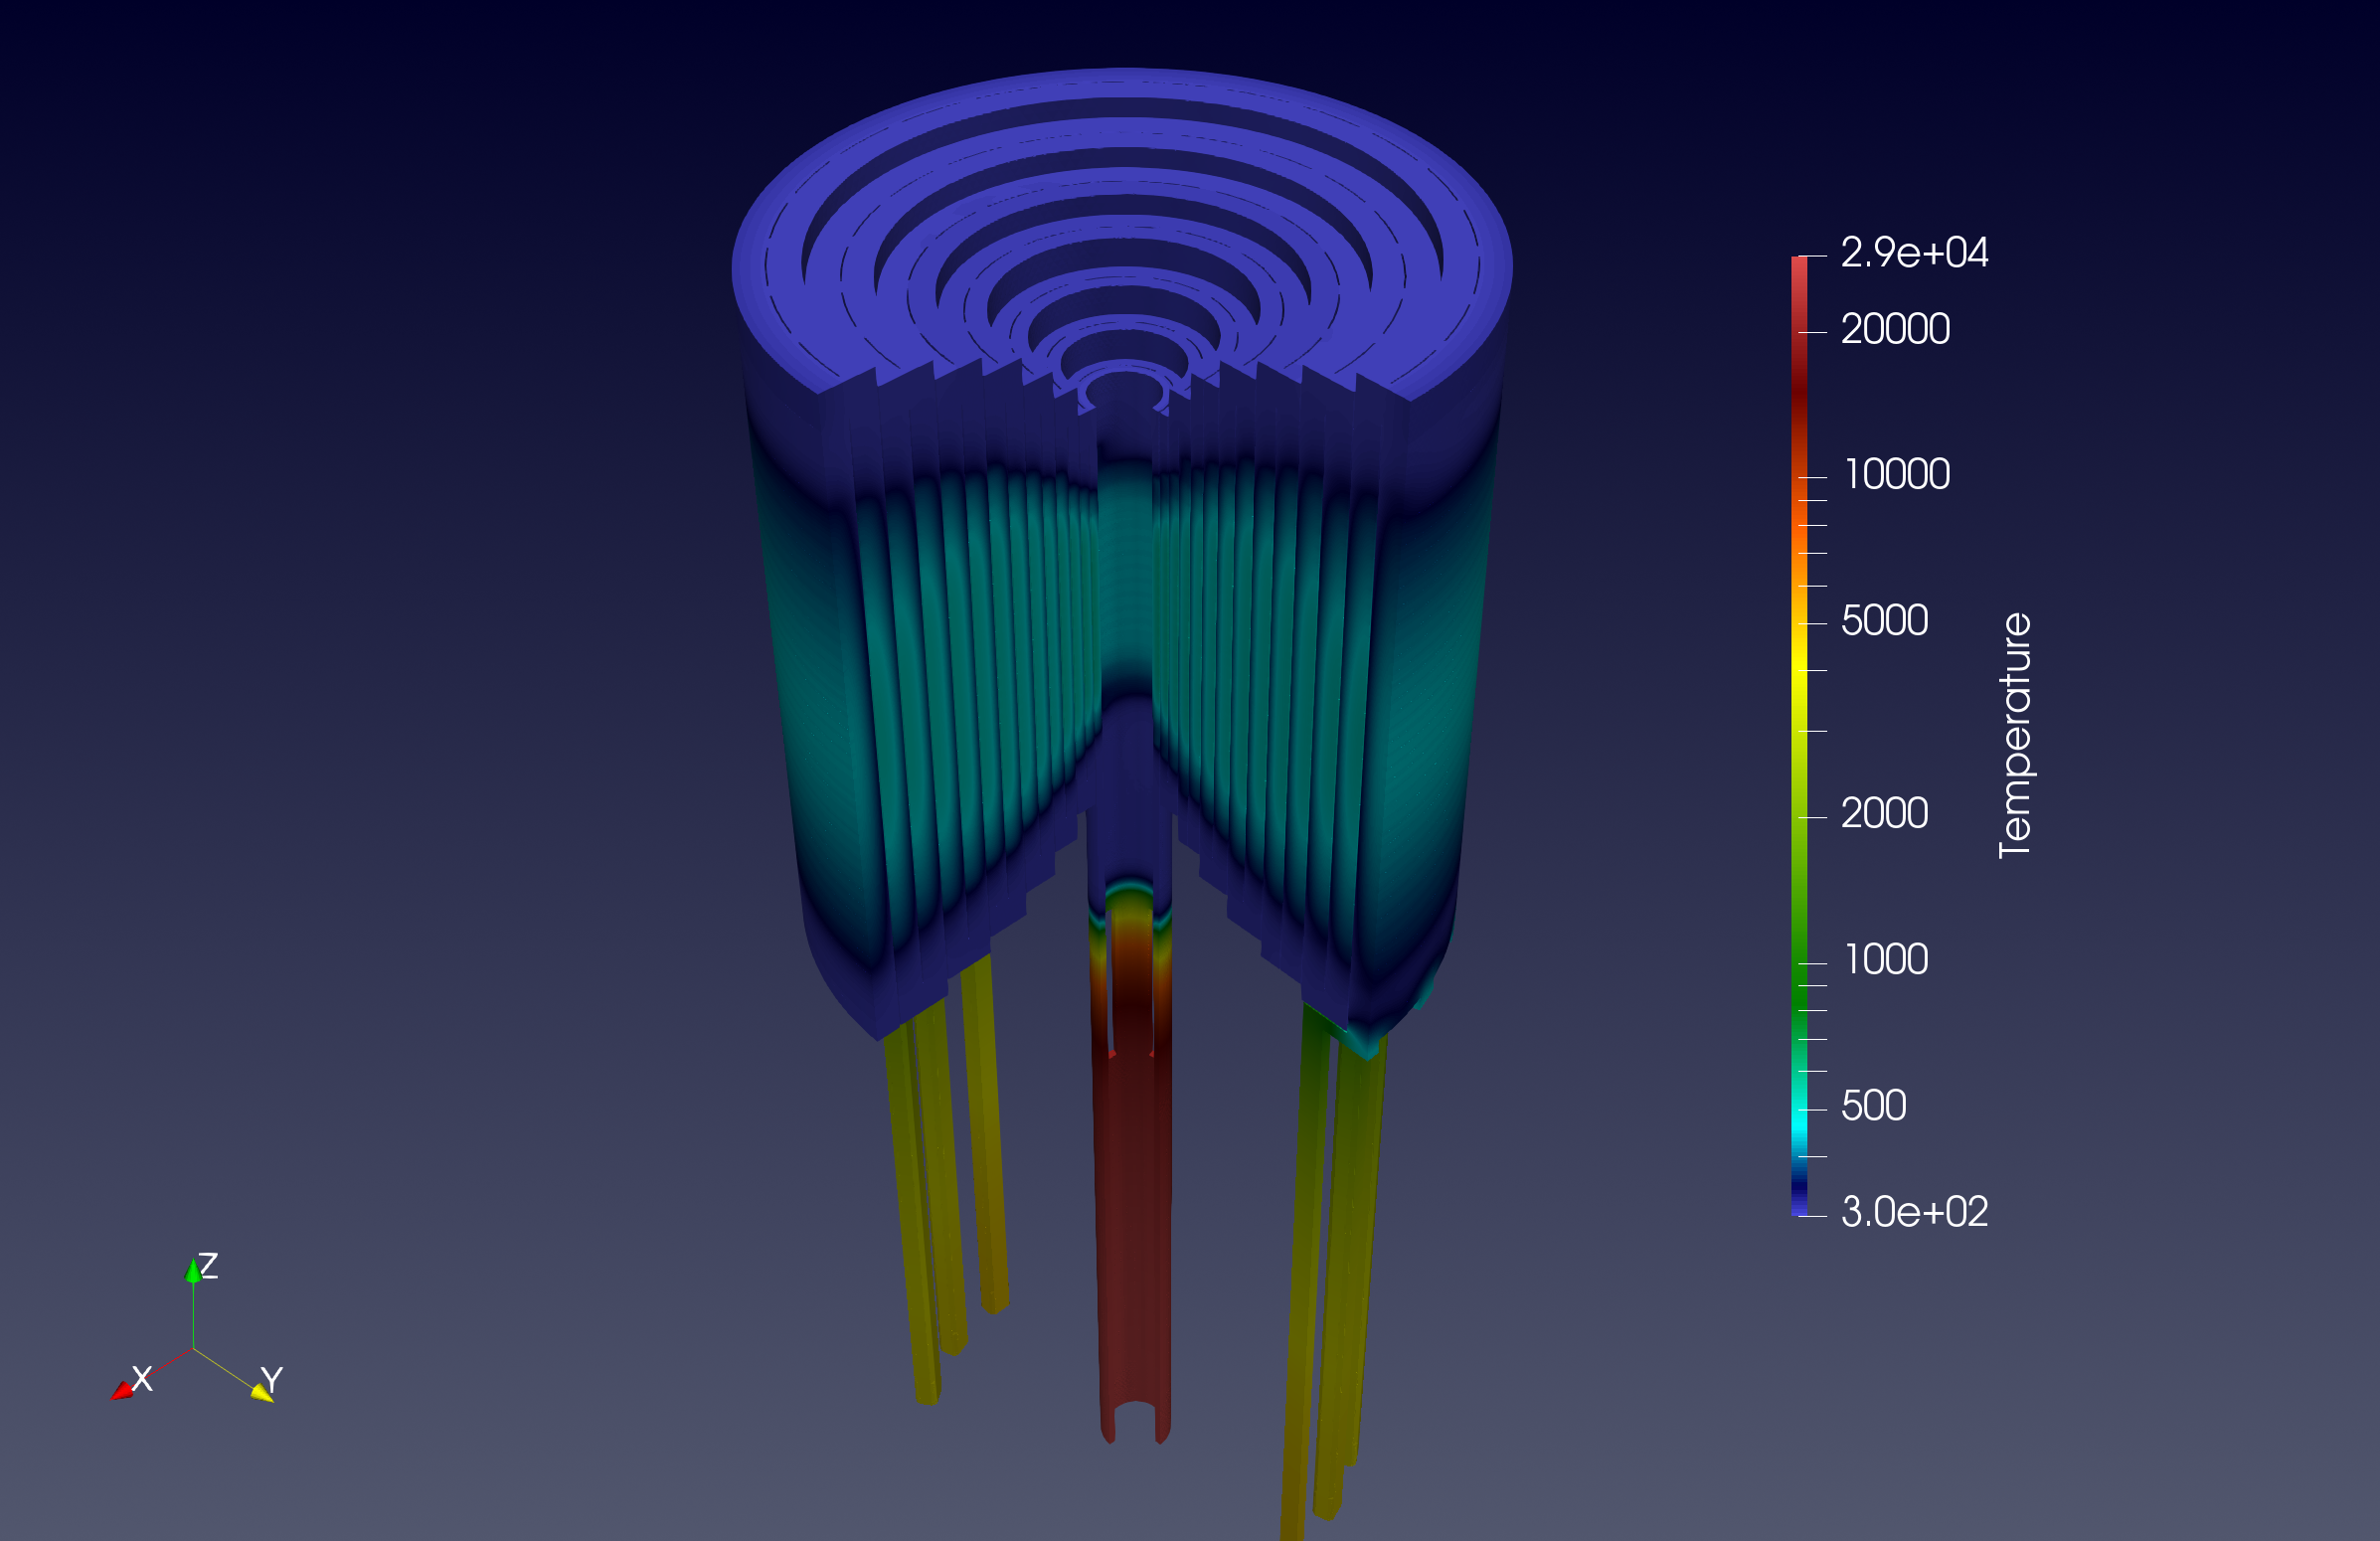
\includegraphics[width=\textwidth]{graphics/feelpp/feelpp-benchmark-HL-31-temperature.png}
    \caption{Temperature}
  \end{subfigure}
  \hfill
  \begin{subfigure}[c]{0.49\textwidth}
    \centering
    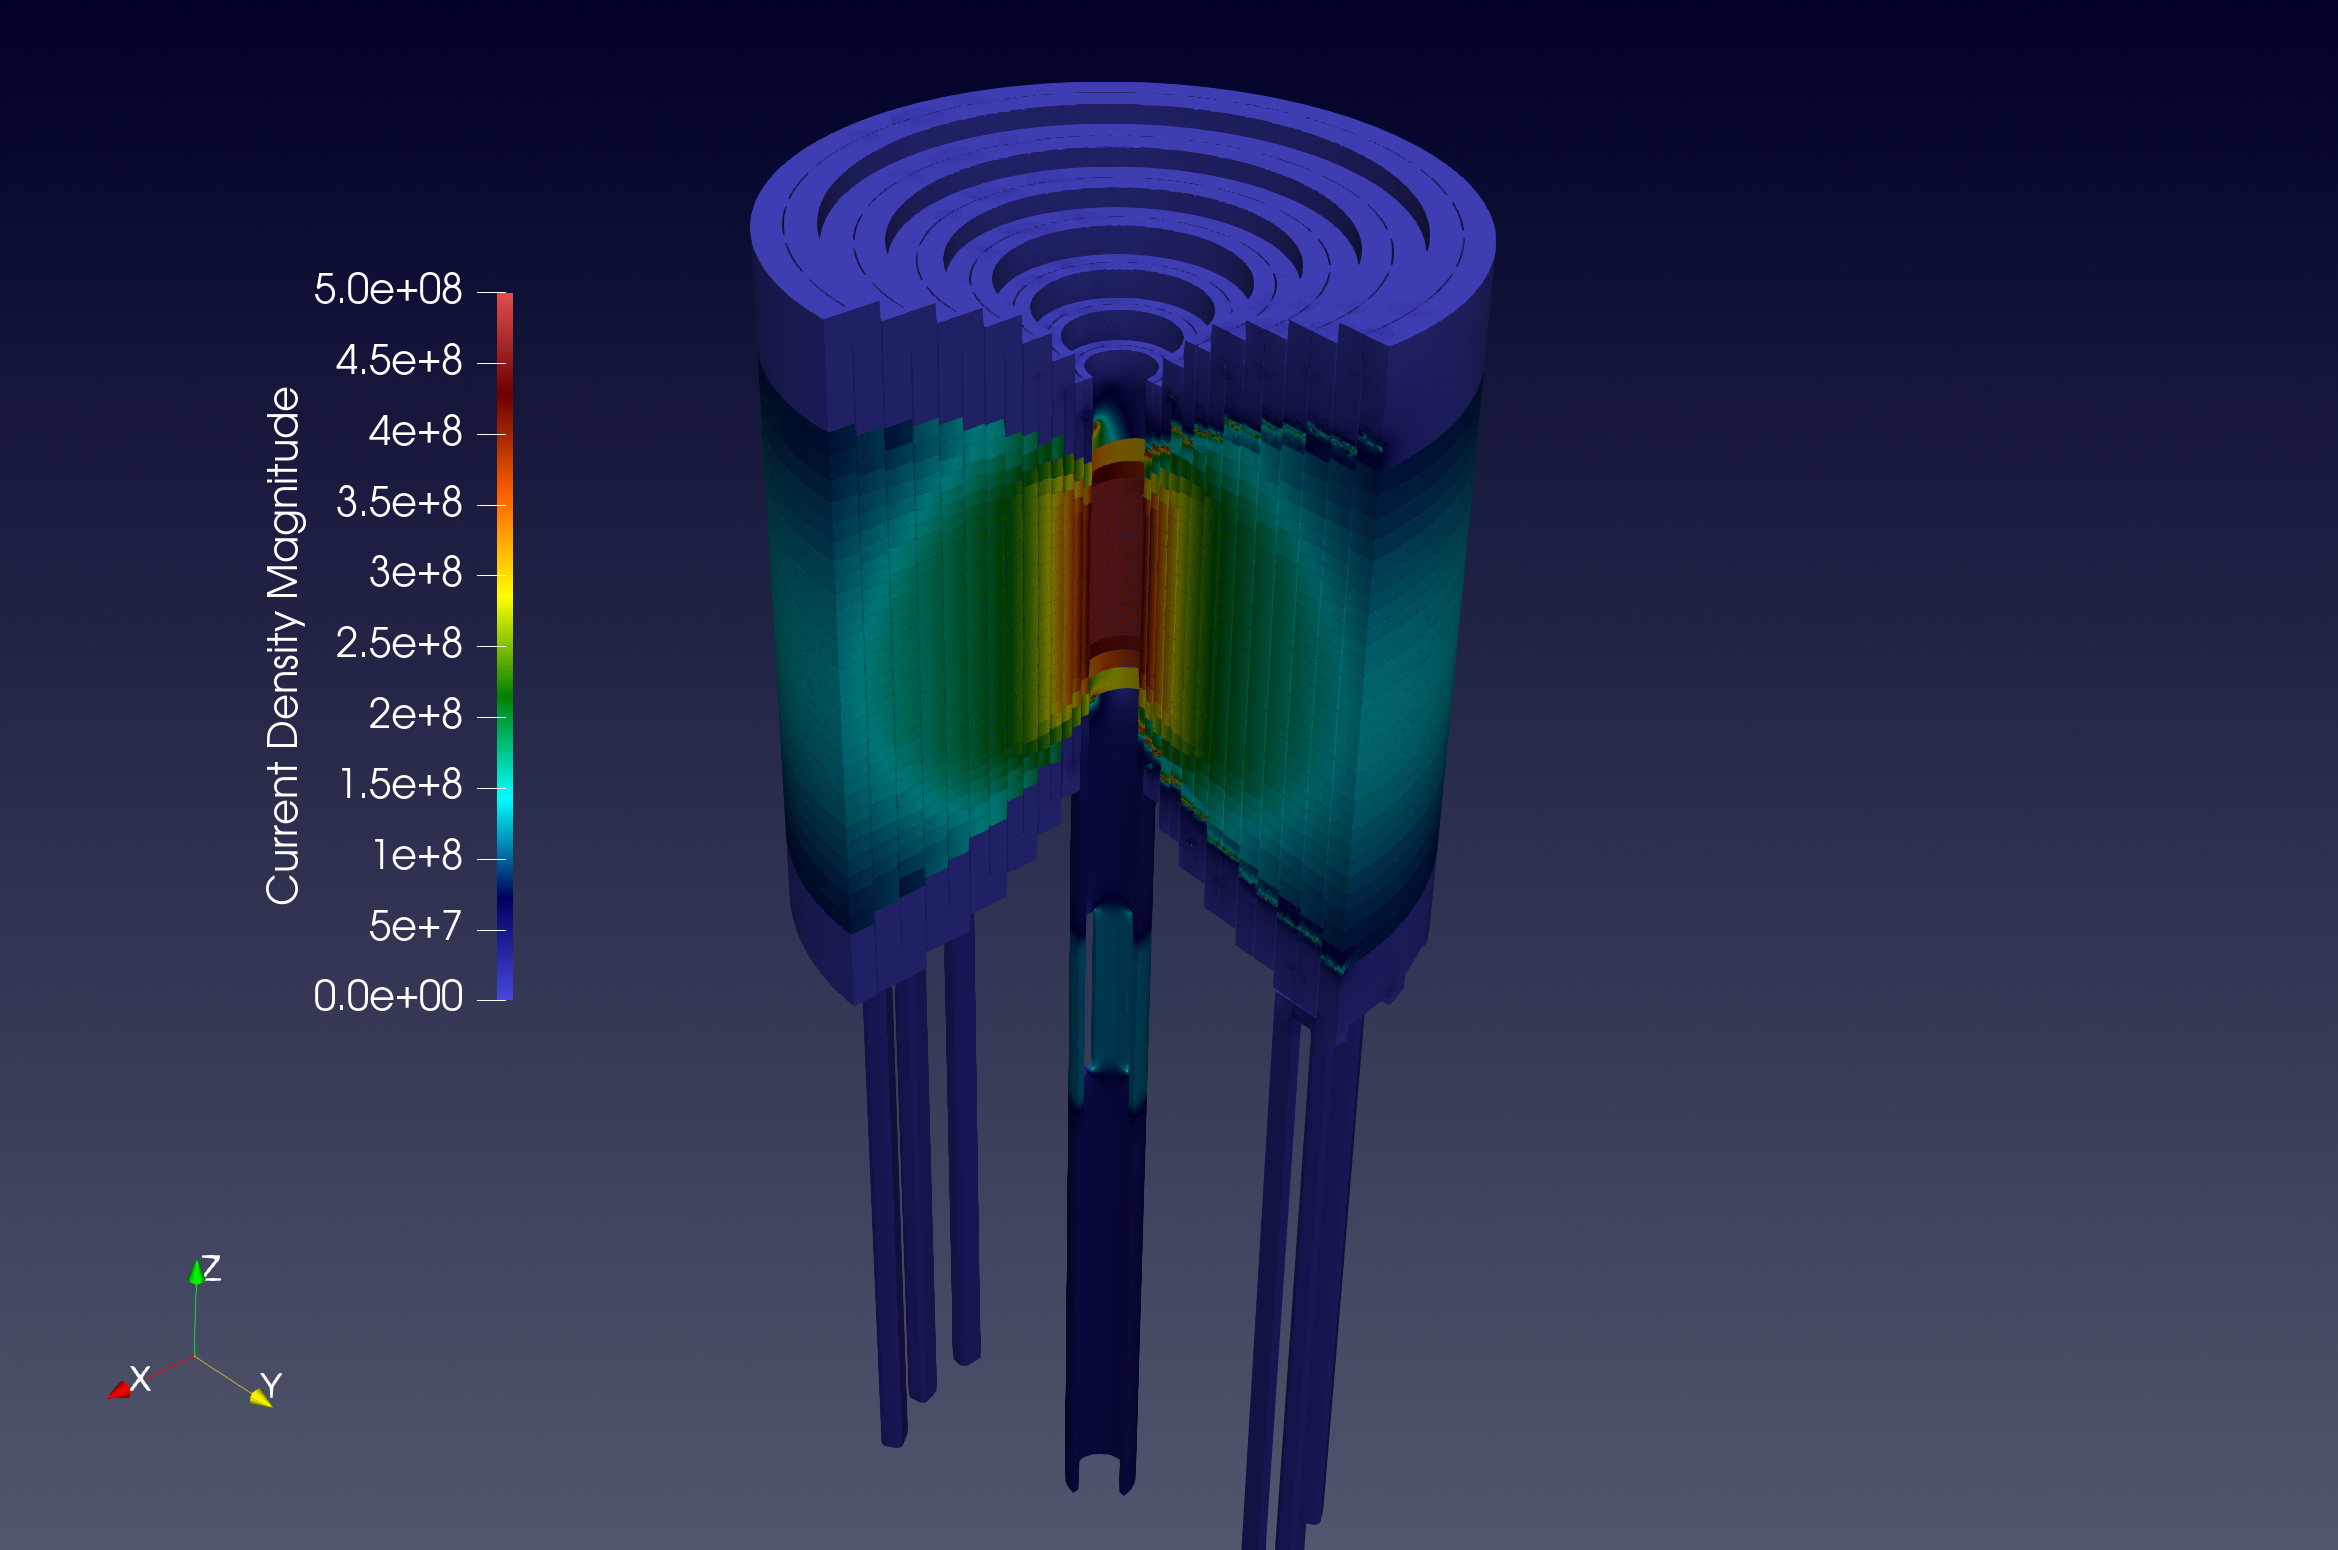
\includegraphics[width=\textwidth]{graphics/feelpp/feelpp-benchmark-HL-31-current_density.png}
    \caption{Current density}
  \end{subfigure}
  \begin{subfigure}[c]{0.49\textwidth}
    \centering
    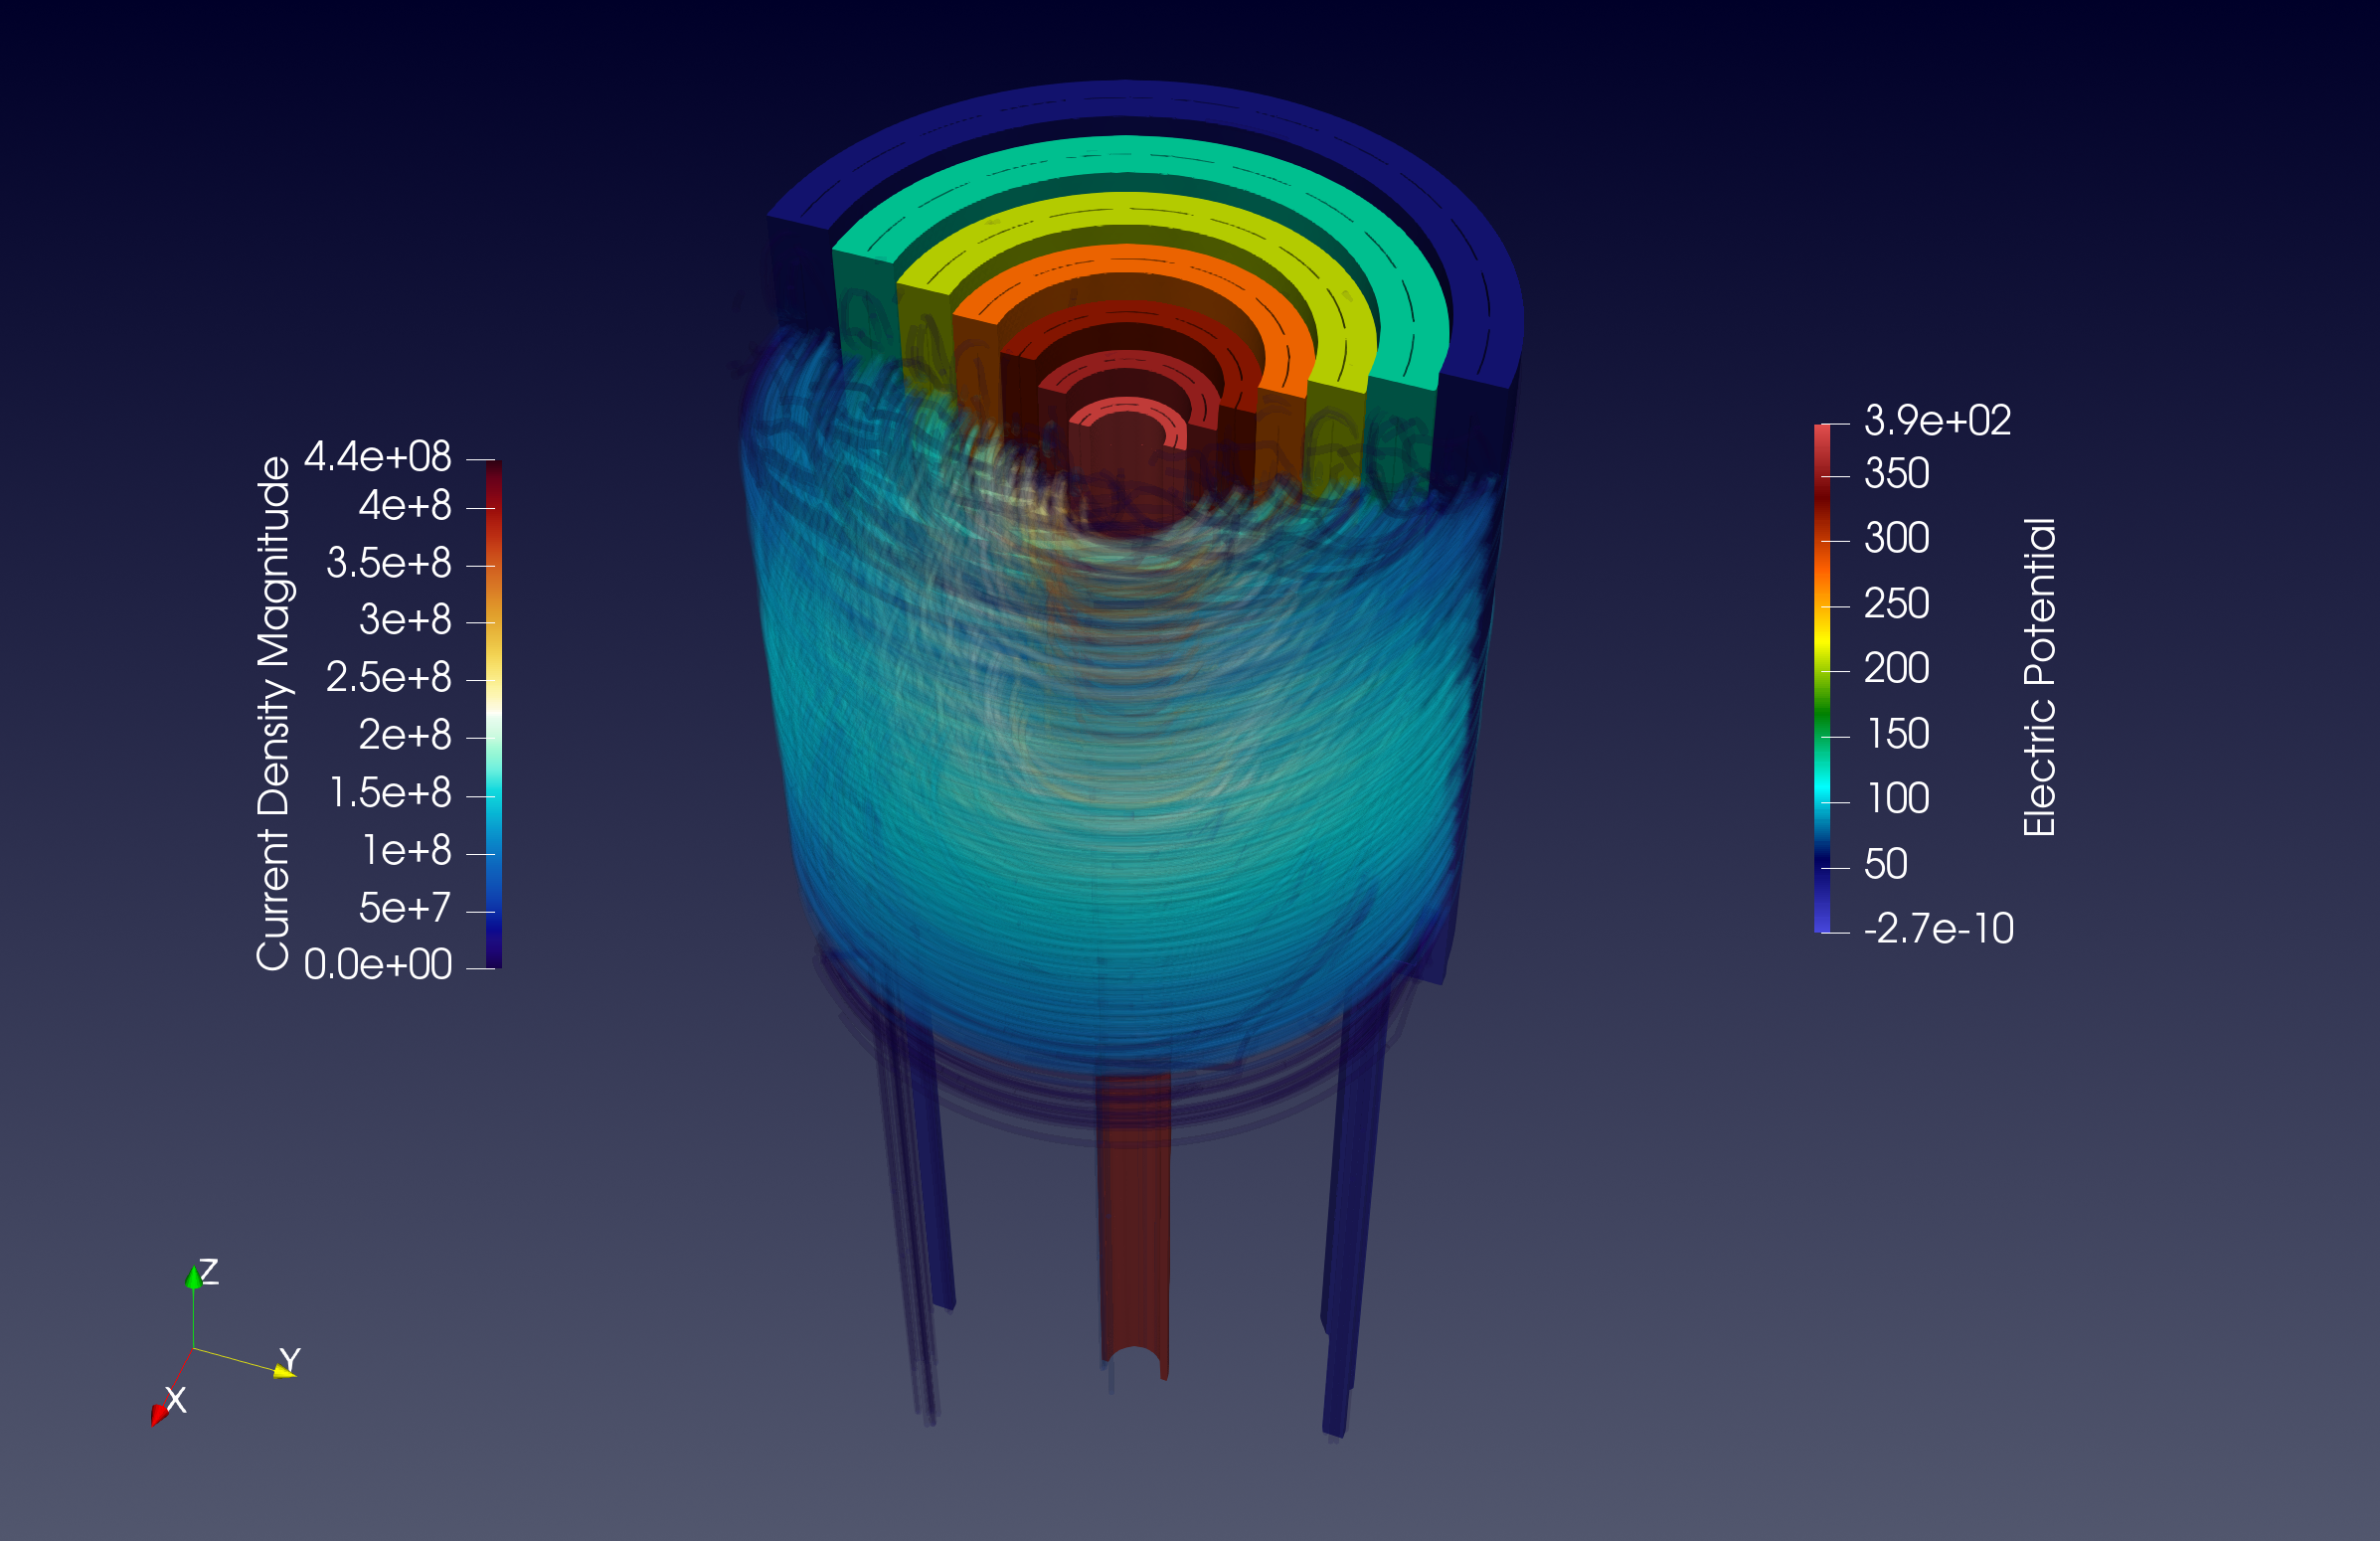
\includegraphics[width=\textwidth]{graphics/feelpp/feelpp-benchmark-HL-31-potential_density_streamines.png}
    \caption{Electric potential and current density on streamlines of electric field}
  \end{subfigure}
  \hfill
  \begin{subfigure}[c]{0.49\textwidth}
    \centering
    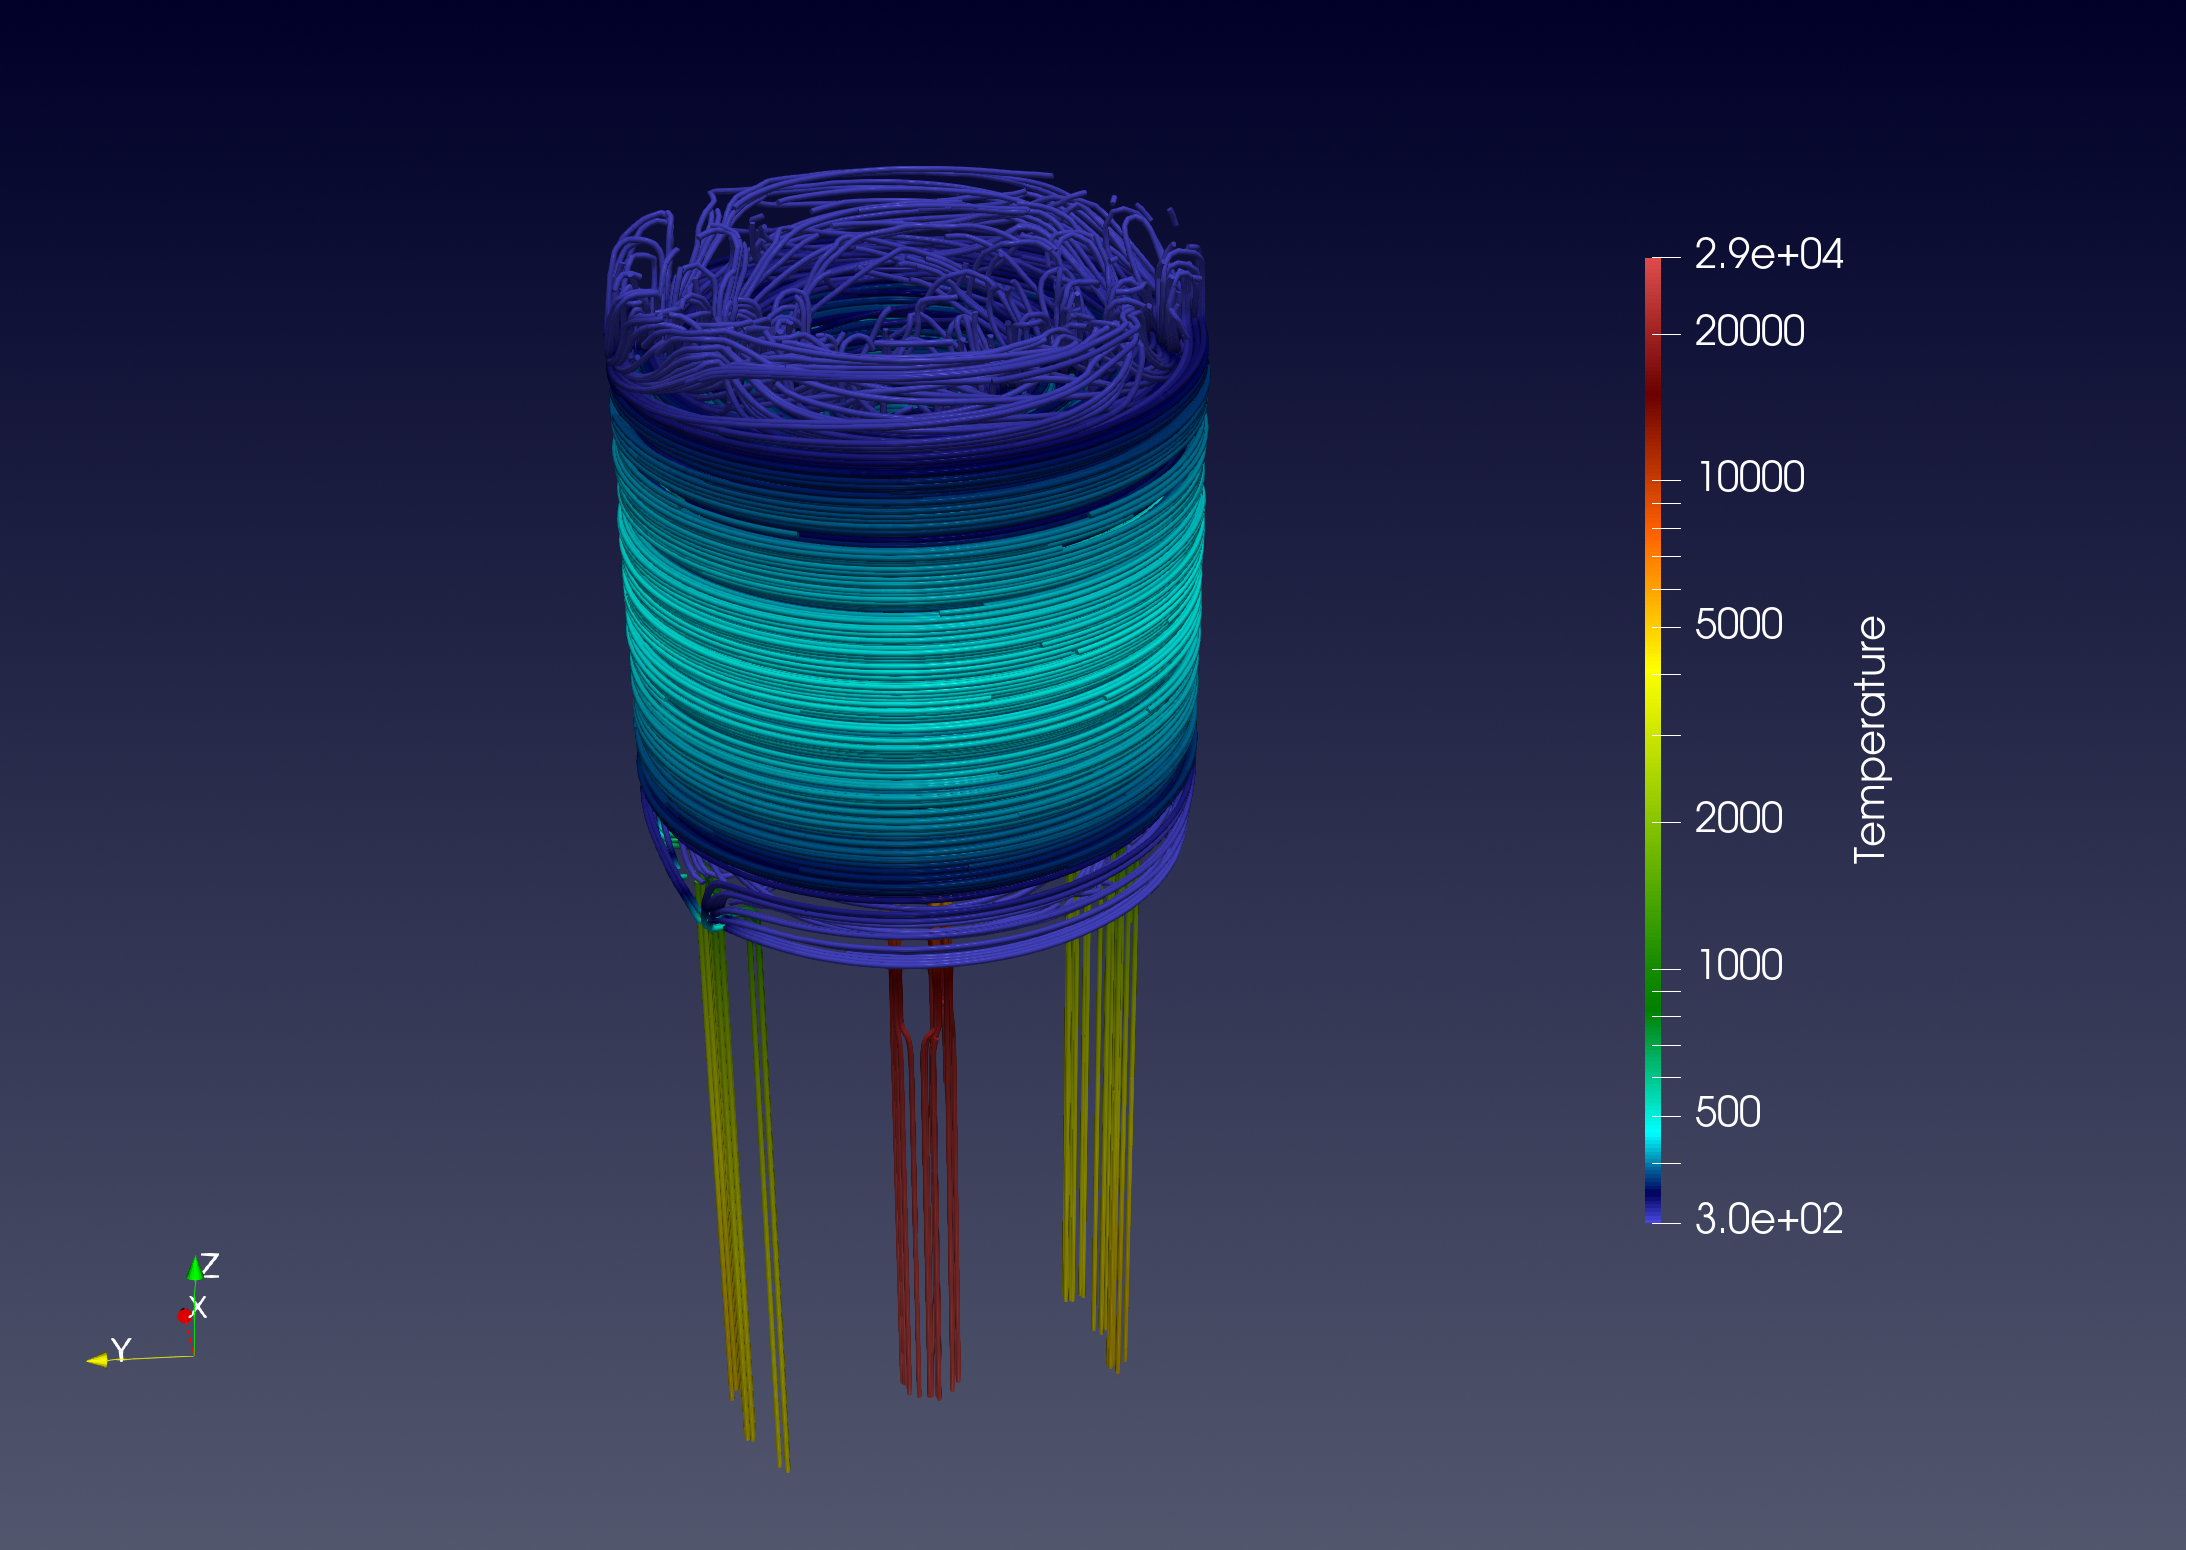
\includegraphics[width=\textwidth]{graphics/feelpp/feelpp-benchmark-HL-31-temperature-streamlines.png}
    \caption{Temperature on streamlines of electric field}
  \end{subfigure}
  \caption{HL-31 benchmarks - solutions}
  \label{fig:spec:app-feelpp:hl-31:results:visualization-solution}
\end{figure}


\foreach [expand list=true] \supercomputerFile/\supercomputerName in {gaya/Gaya} { %,discoverer/Discoverer

  \pgfplotstableread[col sep=comma]{chapters/applications/specs/data/app-feelpp-thermoelectric/exec_times_P1_\supercomputerFile.csv}\dataPa
  \pgfplotstableread[col sep=comma]{chapters/applications/specs/data/app-feelpp-thermoelectric/exec_times_P2_\supercomputerFile.csv}\dataPb
  \pgfplotstableread[col sep=comma]{chapters/applications/specs/data/app-feelpp-thermoelectric/speedup_P1_\supercomputerFile.csv}\dataSpeedupPa
  \pgfplotstableread[col sep=comma]{chapters/applications/specs/data/app-feelpp-thermoelectric/speedup_P2_\supercomputerFile.csv}\dataSpeedupPb

  \begin{figure}[!ht]
    \centering

    \def\chartBarPlot##1##2{
      \barChart[ybar, width=0.97\textwidth, height=0.6172\textwidth,
      xticklabels from table={##2}{tasks},
      x tick label style={ rotate=-45 },
      ylabel={Execution Time (s)},
      legend style={at={(0.5,1.02)}, anchor=south,font=\tiny,legend columns=-1}
      ]{
        {table=##1,column=Init,legend=Init,color=customdarkblue},
        {table=##1,column={Create Mesh},legend={Create Mesh},color=custompurple},
        {table=##1,column=Solve,legend=Assembly,color=customcyan},
        {table=##1,column=Export,legend=PostProcess,color=customorange}
      }
    }

    \def\speedupPlot##1##2{
      \begin{tikzpicture}
        \begin{axis}[
          width=0.97\textwidth, height=0.6172\textwidth,
          ymin=0,
          xlabel={Tasks},
          ylabel={Speedup},
          xtick=data,
          xticklabels from table={##2}{tasks},
          x tick label style={ rotate=-45 },
          xticklabel style={font=\small},
          yticklabel style={font=\small},
          ymajorgrids=true, grid style={dashed, gray!40},
          legend style={at={(0.5,1.02)}, anchor=south, font=\tiny, legend columns=3}
        ]
          % Plot optimal and half-optimal bounds
          \addplot[thick, dashed, color=black] table [x expr=\coordindex, y=optimal] {##2};
          \addlegendentry{Optimal}

          \addplot[thick, dotted, color=black] table [x expr=\coordindex, y=half-optimal] {##2};
          \addlegendentry{Half-optimal}

          % Plot actual speedup
          \addplot[thick, mark=*, mark size=1.5pt, color=customdarkblue] table [x expr=\coordindex, y=Init] {##2};
          \addlegendentry{Init}

          \addplot[thick, mark=square*, mark size=1.5pt, color=custompurple] table [x expr=\coordindex, y={Create Mesh}] {##2};
          \addlegendentry{Create Mesh}

          \addplot[thick, mark=triangle*, mark size=1.5pt, color=customcyan] table [x expr=\coordindex, y=Solve] {##2};
          \addlegendentry{Assembly}

          \addplot[thick, mark=diamond*, mark size=1.5pt, color=customorange] table [x expr=\coordindex, y=Export] {##2};
          \addlegendentry{PostProcess}
        \end{axis}
      \end{tikzpicture}
    }

    \begin{subfigure}[c]{0.49\textwidth}
      \centering
      \chartBarPlot{dataPa}{\dataPa}
      \caption{\texttt{M1} - \texttt{$P_1$} (Execution Time)}
    \end{subfigure}
    \hfill
    \begin{subfigure}[c]{0.49\textwidth}
      \centering
      \speedupPlot{dataSpeedupPa}{\dataSpeedupPa}
      \caption{\texttt{M1} - \texttt{$P_1$} (Speedup)}
    \end{subfigure}

    \vspace*{0.04\textwidth}

    \begin{subfigure}[c]{0.49\textwidth}
      \centering
      \chartBarPlot{dataPb}{\dataPb}
      \caption{\texttt{M1} - \texttt{$P_2$} (Execution Time)}
    \end{subfigure}
    \hfill
    \begin{subfigure}[c]{0.49\textwidth}
      \centering
      \speedupPlot{dataSpeedupPb}{\dataSpeedupPb}
      \caption{\texttt{M1} - \texttt{$P_2$} (Speedup)}
    \end{subfigure}

    \caption{HL-31 benchmarks - Execution time and speedup of main simulation components
      - \supercomputerName \  supercomputer}
    \label{fig:spec:app-feelpp:hl-31:results:performance_times_M1_\supercomputerFile}
  \end{figure}
}


\paragraph{Challenges Identified}

\begin{itemize}
\item HPC experiments with other kinds of discretizations:
  \begin{itemize}
  \item Modelling: nonlinear, Maxwell, ...
  \item HDG method
  \item Geometry complexity
  \end{itemize}
\item Go to extreme HPC scale: Partitioning and IO issues
\end{itemize}

